\documentclass{sig-alternate-05-2015}


\usepackage{cite}
\usepackage{url}
\usepackage{color}
\usepackage{tikz}
\usepackage{balance}
\usepackage{caption}
\usepackage{soul} % Used for highlighting % \hl{this is some highlighted text}
\usepackage{times} % Used for formatting formatting url footnotes
\urlstyle{same} % Used for formatting formatting url footnotes
\usepackage{pgfplots} % Used for bar chart
\usetikzlibrary{patterns} % Used for bar chart
\usetikzlibrary{shapes,arrows} % APK extraction process image
\usepackage{listings}


\setlength\floatsep{1.25\baselineskip plus 3pt minus 2pt}
\setlength\textfloatsep{0.7\baselineskip plus 3pt minus 2pt}
\setlength\intextsep{1.15\baselineskip plus 3pt minus 2 pt}

%%% Messes with the alignment of the table headers
% \RequirePackage[singlelinecheck=off]{caption}
%\captionsetup{justification=centering}

\newcommand{\todo}[1]{\textcolor{cyan}{\textbf{[#1]}}}
\newcommand{\sam}[1]{\textcolor{green}{{\it [Sam says: #1]}}}
\newcommand{\dan}[1]{\textcolor{blue}{{\it [Dan says: #1]}}}
\newcommand{\mei}[1]{\textcolor{red}{{\it [Mei says: #1]}}}



%%%%%%%%%%%%%%%

% Google Docs version
%   https://docs.google.com/document/d/1UWIzcqgGGTT7s__KvJ-Ps2jMmXP-MXisYYB-rZfaOuY/edit?usp=drive_web


\begin{document}

% Mperm: An Android Permission-Gap Detection Tool
% An Android Permissions Gap Detection Tool
% An Android Permissions Analysis Tool for the Updated Permissions Structure
% MPerm: A Tool for Android Permissions Analysis
\title{Most Recent Version in OverLeaf::::M-Perm: An Android Permissions Analysis Tool}



\author{
%
% 1st. author\
\alignauthor
Piper Chester, Cesar Perez and Daniel E. Krutz 	\\
%	\affaddr{Software Engineering Department}\\
       \affaddr{Rochester Institute of Technology, Rochester, NY, USA}\\
       \email{\{pwc1203,cap7879,dxkvse\}@rit.edu}
       \alignauthor
} % Must not be a space above this



\maketitle
\begin{abstract}
Android Applications (apps) operate under a permissions-based system where access to specific APIs are restricted through the use of permissions. Unfortunately, there is no built-in verification system to ensure that apps do not request too many or too few permissions, which could lead to serious quality and/or privacy concerns. Apps requesting too many permissions create unnecessary vulnerabilities, leaving the potential for abuse by SDKs within the app or other malicious apps installed on the device.

With the introduction of Marshmallow 6.0 (M), the Android permission structure has substantially changed from requiring users to accept or reject all permissions when installing the app, to allowing developers to request permissions at run-time. Users also have finer control, gaining the ability to alter individual permissions after installation. Some of the motivating factors for switching to this new model include streamlining the app installation/update process and placing users more in control of the permissions their apps use.

In order to assist with the discovery of under and over-privileges within this new permission structure, we created a new detection tool, \emph{M-Perm}, which can easily and effectively identify permission misuse in Android apps. M-Perm also identifies permission usage in apps including requested normal, dangerous, and 3rd party permissions. The tool, complete usage instructions, and screencast are available on our project website: \url{http://www.m-perm.com}


%% Check to make sure that apps will not crash if they are underprivileged
\end{abstract}


%%% Add  Categories and Subject Descriptors

%% Categories taken from: http://www.jucs.org/ujs/jucs/links/Articles%20by%20Category/D.?mode=bc



%\category{D.4.6}{Operating Systems}Security and Protection;
\category{D.2.4}{SOFTWARE ENGINEERING}Software/Program Verification;

\begin{keywords}
Android, Smartphones, mobile phones, mobile security
\end{keywords}


\section{Introduction}

Android is the world's most popular mobile OS~\cite{OSMarketShare_URL} with over 1.8 million apps available from Google Play alone~\cite{statistica_url}. A cornerstone of Android's security is its use of permissions. Android apps do not have any default permissions associated with them, so the developer must explicitly state the permissions needed by the app. The user must explicitly accept any requested `dangerous' permissions, some of which include the ability to read SMS messages, record audio through the phone's microphone, and access the user's location~\cite{AndroidSystemPermissions_URL}.

% switch this permission with the one below?
Unfortunately, there is no built-in verification system to ensure that apps adhere to the~\emph{principle of least privilege} and do not request unnecessary permissions, which increases the app's attack surface and make it more susceptible to a variety of security and privacy related issues~\cite{johnson2012analysis}. Although tools have been created to detect permission misuse and assist in the permission analysis of Android and its apps~\cite{Au:2012:PAA:2382196.2382222, Felt:2011:APD:2046707.2046779}, no known tools are tailored for the updated Android Marshmallow permission system.

Android Marshmallow 6.0 significantly changed the way Android apps ask the user to accept permissions. In the previous versions of Android, users granted an app's requested permissions at install time in an all or nothing fashion. If the user did not agree to all of the app's requested permissions, they would not be allowed to install the app. In the new permission model, users can decide to only allow the app access to specific permissions, and permissions may be requested at runtime. Users also have the ability to permit or revoke an app's permissions after it has been installed.

In order to detect permission misuse in apps using this new Android permission model, we have created a new publicly available tool~\emph{Marshmallow Permissions Analyzer} (M-Perm) which is available on our project website:~\textbf{\url{http://www.m-perm.com}}. Our tool works by first reverse engineering the Android app (apk) file, and then comparing the permissions requested in the app's source code, against what is defined in the \emph{AndroidManifest.xml} file. A configuration file allows the tool to easily adapt to future alterations in the Android permission structure. M-Perm also reports the app's requested normal, dangerous, and third party permissions.

% Work on this part. I want to make it sound like we did something
We evaluated M-Perm in terms of effectiveness and efficiency against an app oracle with pre-defined instances of permissions misuse, and found that it is able to identify a high level of under and over-privileges in these apps. We also analyzed 50 existing Android apps and found that M-Perm is capable of finding a large number of misused permissions, and other permission related information in these apps.


The rest of the paper is organized as follows: Section~\ref{sec:androidpermissions} provides a background on the Android permission structure and Section~\ref{sec:MPerm} discusses M-Perm and how it works. Section~\ref{sec:evaluation} evaluates M-Perm against a set of 10 oracle apps, and then 50 apps collected from various sources. Section~\ref{sec: toolavailability} describes how to get the tool and Section~\ref{sec: relatedwork} provides a background on related works. Section~\ref{sec: limitations} discusses limitations and future work to be conducted with M-Perm and Section~\ref{sec: conclusion} concludes our study.

%%% Leaving out since I want to cut out comparisons to Stowaway when possible
 %MPerm was also evaluated against a well-known, existing permissions gap analysis tool and found that it performs favorably in terms of effectiveness and efficiency.

%%% If space allows, the paper is organized as follows


%% 6/20: Consider comparing to COPES
%	Maybe make the argument that it is the only tool focused on finding the permission gap using only static analysis, on a computer (not phone)


\newpage
\section{Android Permissions}
\label{sec:androidpermissions}

Android permissions are designed to protect the sensitive resources and information on the device. For example, in order for an app to use a device's camera, it must be granted access to the~\texttt{Camera} permission. There are two primary steps in granting an app permission to use a specific resource. The developer must first tell the app to ask for the permission, which is done in the~\emph{AndroidManfiest.xml} file. Beginning with Marshmallow, the permissions must also be requested in the source code when the app needs access to that specific functionality. The final step in granting an app a permission is for the user to accept or reject this permission when using or installing the app. A primary goal of the Android permission model is to ensure that the user is only granting access to sensitive resources on their device which they are comfortable with.

Android apps created for versions up to, and including Lollipop (API 22) all require the user to accept or reject all permission requests at install time. If the user decided that they did not feel comfortable accepting any of the permissions, they would not be allowed to install, or even update the app if it requested any new permissions. Previous works have criticized the old model of requesting permissions at the beginning of the installation process in an all or nothing fashion for a variety of reasons, including the inability of a user to alter permission settings based on situational constraints such as who is using the device or their location~\cite{Nauman:2010:AEA:1755688.1755732,Conti:2010:CCP:1949317.1949355}. According to Android, some of their primary goals for implementing the new permission model was to streamline the app installation and update process, while providing users more control over the permissions their apps used~\cite{android_developer_URL}. Dangerous permissions in the new model are also associated with groups. For example \texttt{SEND\_SMS} and \texttt{READ\_SMS} are part of the SMS group. If the user accepts any permission in the group, all other permissions in the group are automatically granted~\cite{AndroidSystemPermissions_URL}. Android also allows developers to define their own custom, third party permissions~\cite{Android_Permission_Groups_URL, Android_Permissions_Defined_URL}.

The~\emph{principle of least privilege} is the concept of granting of the least amount of privileges to an application that it needs to properly function~\cite{saltzer1975protection}. Granting extra privileges creates unnecessary security vulnerabilities by allowing malware to abuse these unused permissions, even in benign apps, along with making the app vulnerable to malicious SDKs~\cite{6614340}. These extra privileges also increase the app's attack surface~\cite{Davi:2010:PEA:1949317.1949356, Bartel:2012:ASP:2351676.2351722}.

Previous research has found that Android developers often mistakenly add unnecessary privileges in a counterproductive and futile attempt to make the app work properly, or due to confusion over the permission name~\cite{Felt:2011:APD:2046707.2046779}. In this study, we use the term \emph{overprivilege} to describe a permission setting that grants more than what a developer needs for the task. Likewise, an \emph{underprivilege} is a setting for which the app could fail because it was not given the proper permissions. The primary difference between requested permissions and overprivileges is that requested permissions are merely those that the app asks to use, and does not take into consideration if the app actually needs them or not.

% Likewise, an \emph{underprivilege} is a setting for which the app could fail because it was not given the proper permissions. Overprivileges are considered security risks, underprivileges are frequently considered quality risks.\todo{cite}


\section{M-Perm Tool}
\label{sec:MPerm}

M-Perm is comprised of two primary components, the reverse engineering module and the software analysis component. M-Perm was written in Python to make it accessible to numerous platforms, and to make it more maintainable by others since it is a very popular development language.

\subsection{Reverse Engineering}

The tool is composed of several different Python modules, with each component serving a distinct purpose. The Driver module first initiates the reverse engineering of the target Android APK, using several well known dependencies for APK reverse engineering which have been used in previous research~\cite{Lee_2013,6687155}: dex2jar\footnote{\url{https://code.google.com/p/dex2jar/}}, Apktool\footnote{\url{http://ibotpeaches.github.io/Apktool/}}, and Procyon\footnote{\url{https://bitbucket.org/mstrobel/procyon/}}. The reverse engineering project and scripts exist in a Git submodule within the main repository of the project. We chose to use a Git submodule so updates to the reverse engineering repository can easily be made, which is important since these reverse engineering submodules are regularly updated for routine updates and to handle alterations in Android.


\subsection{App Analysis}

Once the reverse engineering process is completed, the analysis of the app's source code can begin. The Analysis module performs static analysis on the disassembled APK and consists of parsing the application manifest, and then the disassembled source code. The source code analysis portion of M-Perm entails searching through every Java source file, and looking for references of the requested permission. For dangerous permissions, there must be a specific reference to use the permission within source. The analysis module also uses the provided configuration file from the user for grouping and identifying permissions. This configuration file is a text file with permissions and permission groups for the analysis module to ignore. This allows the user to isolate various permission groups during analysis. The analysis component concludes with producing a source report text file of all permission occurrences during analysis.

In the final stage of execution, the Report module examines the source report produced during analysis. This module handles most of the logic for examining which permissions have been requested by the manifest and which permissions are considered dangerous based on their group. Any permissions that occur in the source that were not requested in the manifest are considered underprivileged. Any permissions that didn't occur in the source that were requested in the manifest are considered overprivileged. M-Perm's output are stored in two .txt files in the \emph{reports} directory. An overview of M-Perm's architecture is shown in Figure~\ref{fig:architecture}.


\begin{figure}[ht!]
\centering
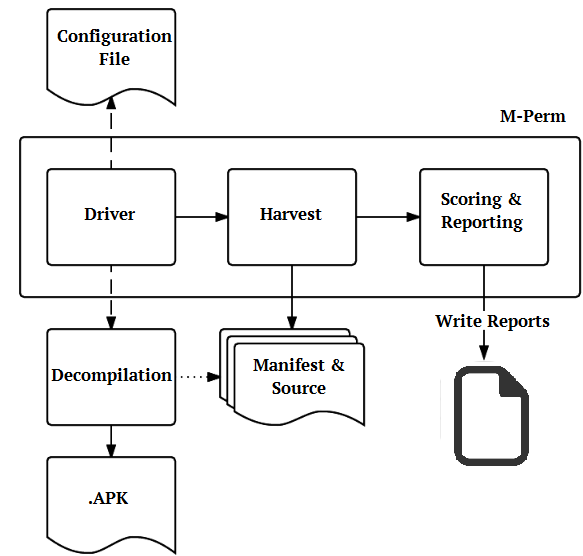
\includegraphics[width=\columnwidth, angle = 0, scale=.99]{images/architecture.png}
\caption{M-Perm Architecture} % \todo{make into latex}
\label{fig:architecture}
\end{figure}


The Android permission structure regularly changes, and unfortunately these alterations often have a negative impact on a tool's ability to effectively examine an app's permissions. In order to accommodate change, M-Perm relies upon a configuration file \emph{Permissions.py}, which holds the permission structure of the targeted Android OS. This file contains Android's dangerous and normal permissions, along with their defined groups. We plan on regularly updating this configuration file in our version control system to meet the changing structure of the Android permission system, although it should not be difficult for the typical developer to configure on their own as they desire.


%%% If there are not many technical challenges, then just roll this section up into another
%\subsection{Technical Challenges}
%\label{sec:technicalChallenges}

%\todo{Do this part}


%%% Address some of the weaknesses we state later on in the work

%% Sell it to make it seem difficult


% Creating a tool which is capable of analyzing a diverse set of Android apps written in a diverse manner is difficult


%One of the primary benefits of Android is its diversity to run on numerous devices,




%% Ensuring that the decompliation process would work


%% Creating a system that was easily extensible and that would grow over time

%% Run time vs. Install time

%%



%The biggest technical challenges we saw during the tool?s development were the inconsistencies with third party dependencies. Because the tool relies on a set of third party decompilation libraries, including dex2jar, apktool, etc. We had inconsistencies with decompilation across versions. We needed to freeze the version in order to guarantee that we wouldn?t have any inconsistencies.

%Another challenge we faced was that no one had previously addressed M permissions in an analysis tool. This involved learning about the M permissions runtime system which is different than previous install time permission systems of Android.

%Part of the reasoning behind choosing Python as the primary language for the tool was the maintainability and readability of it. Prior Android permission tools were very difficult to start using, largely because of little documentation and unmaintainable code. With Python, we encourage and hope that members of the open source community to contribute to and improve the tool. The barrier to entry is low, and the majority of the source of the tool is self-documenting and very readable.




\subsection{Tool Output} % Come up with a better name
% Have this section? Talk about some of the items that can be used from the output

Once completed, M-Perm's output is placed inside of two .txt files. The first is~\texttt{analysis\_<package\_name>} which lists the normal, dangerous, 3rd party, and under \& over privileges found in the app. The file also correlates the requested dangerous permissions with their associated permission groups, along with all dangerous permissions in the app and how they are being used. For example, dangerous permissions may be directly used by the app in a function, or the app may merely check to see if the app already has access to the permission. M-Perm will provide the context of how the app is using this permission. Knowing the context of permission requests can be useful to a variety of researchers including those analyzing app permission leaks~\cite{wang2015cicc}, or those simply looking to better understand app permissions and how they are used.

The second file~\texttt{source\_report\_<package\_name>}, goes into more detail describing the usage of permissions inside of the app. The report lists the files that permission requests occur in, along with the block of code that is requesting the permission. For example, a permission snippet in this file could include an error or log message, checking to see if a permission has been granted, or even built in checks for possible malicious app usage. This output may be useful for both developers and researchers who would like to learn more about permission usage in either individual apps, or may be performed on a large set of apps to create a larger, aggregate data set. % Might be a good idea to give specific information about permission usage.


%%% Show this as a snippet if space is an issue
%File:  sample_apks/cnn.apk.uncompressed//app/src/android/support/v7/app/TwilightManager.java
%
%        final int checkSelfPermission = PermissionChecker.checkSelfPermission(this.mContext, "android.permission.ACCESS_COARSE_LOCATION");
%        final int checkSelfPermission2 = PermissionChecker.checkSelfPermission(this.mContext, "android.permission.ACCESS_FINE_LOCATION");
%        Log.i("TwilightManager", "Could not get last known location. This is probably because the app does not have any location permissions. Falling back to hardcoded sunrise/sunset values.");



%%% This is important because...


Further documentation on the rest of these output files, along with other useful M-Perm information may be found on the project website.


%%% Show image with the output in it?


\section{Evaluation}
\label{sec:evaluation}

In order to assess the effectiveness and efficiency of M-Perm, we first evaluated it against a small set of oracle apps that we created specifically for this study. These apps contained pre-defined over and under permissions. We chose to evaluate M-Perm on several criteria including effectiveness (Precision, Accuracy, F-score \& Accuracy), adaptability, and analysis time. In several cases, we compared M-Perm against Stowaway~\cite{Felt:2011:APD:2046707.2046779}, a well-known Android Permission analysis tool. Although Stowaway was once likely regarded as the most effective tool for detecting permission gaps in Android apps, it is unfortunately several Android versions out of date, and according to its own website will likely produce inaccurate results. However, we still chose to display the results of M-Perm against Stowaway since it is likely the most well-known permission analysis tool with over 800 citations, and that it is a freely available open source tool.


\textbf{Effectiveness: }There are several ways to evaluate a program's effectiveness, including measuring the precision, recall, accuracy and F-score of the tool. Before the completion of M-Perm, we created an oracle set of apps to test the effectiveness of the permission analysis portion of the tool. This included 5 APKs that referenced the permissions that were requested in the manifest, and 5 APKs that did not reference the permissions that were requested in the manifest. The permissions we tested for included \texttt{READ\_CALENDAR}, \texttt{ACCESS\_FINE\_LOCATION} , \texttt{CAMERA}, \\ \texttt{READ\_CONTACTS}, and
\texttt{SEND\_SMS}; all permissions which are considered to be `dangerous', and must be requested directly by the app for them to be used.  We chose to create an oracle since we could more easily and accurately control permission usage in sample apps which we created. Since M-Perm only works on Marshmallow 6.0 or above apps, all created apps were targeted for API 23. We then ran both Stowaway and M-Perm on this oracle of apps and evaluated their effectiveness in properly identifying over and under permissions. These results are shown in Figure~\ref{fig:toolcomparision}.

\definecolor{bblue}{HTML}{4F81BD}
\definecolor{rred}{HTML}{C0504D}
\definecolor{ggreen}{HTML}{9BBB59}
\definecolor{ppurple}{HTML}{9F4C7C}

\begin{center}

\begin{tabular}{@{}lp{4cm}}
\resizebox {\columnwidth} {!} {
\begin{tikzpicture}
    \begin{axis}[
        width  = .5*\textwidth,
        height = 6cm,
	   legend style={at={(0.50,0.42)},anchor=north}, % Right left/Up Down
%        major x tick style = transparent,
        ybar,
%        bar width=8pt,
%        ymajorgrids = true,
%	xlabel={Measurment Tools},
%    nodes near coords,                     %% new
%    nodes near coords align={vertical},    %% new
    enlarge x limits={abs=1.5cm},   % align the bars
%	ylabel = {Score},
	ymin=0,ymax=1.0,
        symbolic x coords={Stowaway,M-Perm},
        xtick = data,
        scaled y ticks = false,
    ]

	% Precision
  	\addplot[style={bblue,fill=bblue,mark=none}]  coordinates {(Stowaway, .75) (M-Perm,1.00)};

	% Recall
   	\addplot[style={rred,fill=rred,mark=none}] coordinates {(Stowaway, 1.00) (M-Perm,1.00)};

	% F-score
     	\addplot[style={ggreen,fill=ggreen,mark=none}]  coordinates {(Stowaway, .50) (M-Perm,1.00)};

	% Accuracy
       	\addplot[style={ppurple,fill=ppurple,mark=none}]   coordinates {(Stowaway, .8333) (M-Perm,1.00)};


     \legend{Precision,Recall,F-score,Accuracy}

    \end{axis}

\end{tikzpicture}
}
\end{tabular}
	\captionof{figure}{Tool Comparison on Oracle Apps}
	\label{fig:toolcomparision}
\end{center}

%What we found that Stowaway considered both the No Reference and the Reference permission apps to be overprivileged, whereas MPerm didn't consider the oracle apps with reference permissions to be over privileged, as we reference them in the source.

These results demonstrate the effectiveness of M-Perm to discover misused permissions in a small set of 10 custom apps in terms of precision, recall, accuracy and F-score.


Our next goal was to evaluate M-Perm on a larger set of exsiting Android apps. We began by collecting 50 apps targeted for Android Marshmallow from both Google Play\footnote{\url{https://play.google.com/}} and apkMirror\footnote{\url{https://www.apkmirror.com}}. A few of these apps included Uber, Skype, LinkedIn, Twitter, and Google Calendar. We next examined each of these apps using M-Perm with the goal of ensuring that the tool was able to collect a variety of permissions related information about each app. The results of this analysis are shown in Table~\ref{Table:appAnalysisResults}.


%% Tended to stick with more well known apps


\begin{table}[ht]% Try here, and then top
\begin{center}
\caption{Analysis Results for 50 Apps}
\label{Table:appAnalysisResults}
  \begin{tabular}{ l | l  | l }

    \bfseries  & \bfseries Total & \bfseries avg/App \\ \hline
    Total Permissions & 1119 & 22.4  \\ \hline
    Dangerous Permissions & 531  & 10.6 \\ \hline
    Third Party Permissions& 321 & 6.4 \\ \hline
    Under Privileges & 89 & 1.8 \\ \hline
    Over Privileges & 110 & 2.2 \\

  \end{tabular}
  \end{center}
\end{table}



Previous research has found that roughly a third of all apps contain at least one overprivilege~\cite{Felt:2011:APD:2046707.2046779}. In our very limited analysis, we found that less than 20\% of collected apps contained an overprivilege, which indicates that the overprivilege rate is dropping in Android M apps using the new permission structure. However, our sample size is very small, and calls for future work in this area.

Although far from a comprehensive study, our brief analysis demonstrates the capabilities of M-Perm along with serving as an indicator that the permission gap is still an issue in the reorganized permission model.




%\todo{add in a short statement about this}


%	Total Permissions -- table?
%		Dangerous
%		Groups
%		Normal
%		3rd Party



%   Goal was to merely show that MPerm could find over and underprivs in this oracle of apps, even if Stowaway is no longer as effective as it once ways, it does show that MPerm is an effective tool for discovering over and under privs.







\textbf{Adaptability:} Future changes to the Android OS and its permission structure are inevitable. Therefore, it is imperative to create tools which can easily grow and adapt with Android. An important goal of our tool was to ensure that it was effective not only for the current version of Android M (6.0), but would also an effective tool with future versions of Android as well. M-Perm relies upon an app configuration file in order to identify \emph{Normal} and \emph{Dangerous} permissions, along with the groups which they belong to. This configuration file should make M-Perm easily adaptable for unforeseen permissions and grouping changes in future offerings of the Android OS.

\textbf{Speed:} Whether analyzing one app, or one thousand apps, the speed of an analysis tool is important. The vast majority of analysis time required by M-Perm was due to the reverse engineering process. For example, the Uber app took 288 seconds to be disassembled from an apk to .java source code, but took only about one second for M-Perm to analyze and create the final reports. We recorded the time required to complete the entire M-Perm analysis for each of the 50 real-world Android apps. On average, it took 328 seconds to complete the entire analysis process, with the shortest app taking 87 seconds to complete, and the longest taking 775 seconds. We expect that future improvements in the reverse engineering process will help to make the tool faster. However, it should be noted that numerous Android static analysis tools take much longer to complete. For example, components of PScout~\cite{Au:2012:PAA:2382196.2382222} are noted to take approximately half a day to complete~\cite{PScout_GitHUb_URL}.



%	Since the app is comprised of two components with a low amount of coupling, altering/updating the reverse engineering module should be very straightforward
%	Show a scatter plot? How do other tools show time?
% 	What were some reasons why Mperm worked better or worse than the other tools?
%	Time to execute tools


\section{Tool Availability}
\label{sec: toolavailability}

M-Perm is publicly available on our project website:~\textbf{\url{http://www.m-perm.com}}. Our site contains the application, information on how to use the tool, and a link to the source code which is available on our GitHub page. We have also created a step-by-step guide for using our tool. Although we believe our tool has an easy to follow installation process, we have also made our tool available for download in a Ubuntu 16.04 LTS Virtual Machine (VM) which is available on our project website. We encourage first time users of M-Perm to use the tool through this provided VM.


%%% Can probably remove this section if there is not room. Most other papers don't have it
\section{Related Work}
\label{sec: relatedwork}



%%% COPES: Automatically Securing Permission-Based Software by Reducing the Attack Surface: An Application to Android

%% Interesting snippet on PScout => http://stackoverflow.com/questions/24858462/how-to-check-if-android-permission-is-actually-being-used

"PScout does a better job than Stowaway at generating the permission maps. However, PScout does not include an APK analyzer, so you will have to manually compare the mappings they provide with API calls made by your app."


%	6/19 - After publishing
% A few other possible works to take a look at:
%	> Reevaluating Android Permission Gaps with Static and Dynamic Analysis
%	6/20
%       http://siis.cse.psu.edu/ded/ > A decompiling link.

%   6/20 -> The tool only finds dangerous permissions - If the non-dangerous permissions are never requested, we will never search for them. How could we find these?
%   


%%% What works are out there that show the dangerous of overprivs

%The topic of reducing the permission gap in Android applications has received a considerable amount of attention recent years. Much of the existing work in this area has dealt with ways of reducing these unneeded permissions and the security vulnerabilities they may lead to. Jeon~\emph{et al.} introduced a framework for creating finer-grained permissions in Android. They believe that the course-grained permissions currently used by Android limit developers by forcing them to choose all of the permissions located in each ``bucket'' when they really only want to add a few of them. This leads to applications having many more permissions than they actually require. The authors believe that finer-grained permissions would lead to only having the needed permissions used by an application, and thus would lead to few vulnerability possibilities~\cite{jeon2011dr}


The dangers of the Android permissions gap has received considerable attention over the last few years. In 2011 Felt~\emph{et al.}\cite{Felt:2011:APD:2046707.2046779} surveyed 940 apps from the Android market and found that about one-third of apps contained at least one overprivilege. Wu~\emph{et al.}\cite{Wu:2013:IVC:2508859.2516728} found that vendor customizations on Android devices contain a significant amount of security vulnerabilities, largely due to 85\% of all pre-loaded apps in stock images containing overprivileges. Wei~\emph{et al.}\cite{Wei:2012:PEA:2420950.2420956} analyzed third party and pre-installed Android apps and found that a high number of apps violated the principle of least privilege and that apps tend to add more privileges with each released version. %%% Add another item to this list if space allows

%% Why do overprivs occur. What causes them? Developer issues?
Felt~\emph{et al.}\cite{Felt:2011:APD:2046707.2046779} conducted research to determine the cause of the permission gap and found that Android developers often mistakenly add unnecessary privileges in a counterproductive and futile attempt to make the app work properly, or due to confusion over the permission name they add it incorrectly believing its functionality is necessary for their app.


%%% Now discuss the tools which talk about overprivs
Although M-Perm is the first permission analysis tool directly targeted towards the new Android permission model, there are several tools which have been developed to assist in the decision making, permission process for developers. Stowaway is a powerful static analysis tool which has been used in previous research~\cite{Pearce:2012:APS:2414456.2414498,Stevens_investigatinguser,jeon2011dr}, but it does suffer from drawbacks. Stowaway's own authors state that the tool only achieves 85\% code coverage~\cite{Felt:2011:APD:2046707.2046779}. Additionally, the tool does not appear to have been modified to support more recent versions of the Android API.

Stowaway and PScout~\cite{Au:2012:PAA:2382196.2382222} both analyze the Android permission systems and provide a permission-API mapping using static analysis. Pscout has been used in several areas including the creation of a list of system calls requiring permissions~\cite{book2013longitudinal,6693128}, research on privilege escalation attacks~\cite{Au:2012:PAA:2382196.2382222}, and assisting with app risk assessments~\cite{pandita2013whyper}. Unlike M-Perm, PScout is not intended to run on specific Android apps. The goal of PScout is to extract the mappings between the permissions defined in the Android operating system, and its API calls defined in primary jar files. Permlyzer is a tool which was built to determine where permissions are utilized in Android applications by using a mixture of static and runtime analysis~\cite{6698893}.

%Mining Android Apps to Recommend Permissions

% Au K W Y et al.[11] developed PScout, a tool that extracts the permission specification from the Android OS source code using static analysis. They used PScout to analyze 4 versions of Android and found that if applications only use documented APIs, then about 22% of the non-system permissions are actually unnecessary.



%Although their primary goal is to not examine apps for permission gaps, there are a variety of other Android tools which are associated with permissions analysis.


%While the authors of this tool were able to achieve promising results, subsequent work has criticized this tool for not being accurate enough, since Android's permissions could be different at runtime --- something the tool is not capable of discovering~\cite{zhang2013vetting}.

%We did not perform a direct comparison with our tool and Pscout because.....


%%% Look into Androguard > http://docs.koodous.com/yara/androguard/

%   Does not support Marshmallow
%

%%% Look into StaDynA > http://www.zhauniarovich.com/files/pubs/Stadyna_Zhauniarovich2015.pdf



% https://github.com/Xbalien/vetdroid


%%%% Citations in: https://raw.githubusercontent.com/dan7800/Research/master/Research_Bucket/Completed_Archived/rejected/sac2016/static_analysis_stats/AndroidData.bib

%   Stowaway - 85%. Out of date
%




%%% Future work section?
\section{Limitations \& Future Work}
\label{sec: limitations}

One of the most significant limitations of M-Perm is that it only works with Android M 6.0 apps and higher. Although this represents the future direction of Android, many apps have yet to be converted to use the new model and only 10\% of current Android devices are running Marshmallow~\cite{Mars_Adoption_10_URL}. This low conversation rate is not surprising due to Android's fragmentation problem~\cite{acar2016sok}.

M-Perm is largely dependent on 3rd party tools for reverse engineering target apps. These external tools frequently suffer issues which prevent extracting the necessary functionality from these apps, which limits the effectiveness of M-Perm. Future improvements may be made to increase both the speed, and quality of the reverse engineering process. It is also not fully understood how M-Perm will work with all variations of obfuscated code, although no known issues have been encountered thus far.


A primary goal for the development of the tool was to apply it to a large scale study to analyze permission usage in Android apps. The tool was designed to be robust, easily extensible, and fast. In conjunction with the use of existing tools, future work may be conducted to analyze a large number of Android apps collected from various locations such as Google Play, the Amazon app store\footnote{\url{www.amazon.com/appstore}}, F-Droid\footnote{\url{https://f-droid.org/}}, and AppsAPK\footnote{\url{http://www.appsapk.com/}} to conduct such work as comparing the rates of over and under privileges between Pre-M and Marshmallow apps, which has likely changed due to the reorganization of this permission model



%   Only works on M-apps
%   More robust evaluation (against other apps and against more Google Apps)
%   Perform a large scale study using the tool. See how much the new permission model affects over and under privs
%   Larger Creation of Android oracle
%	Apply the tool to other areas of security. Malware?






\section{Conclusion}
\label{sec: conclusion}

We have created an Android permission analysis tool, M-Perm, which is able to identify permission usage and permission gap issues in the new Android permission structure. We evaluated our tool against 10 oracle apps and found that it is able to both correctly identify permission gap issues in these apps, and how the permissions are used as well. We also evaluated our tool against 50 publicly available apps collected from the web. M-Perm is available on our project website:~\textbf{\url{http://www.m-perm.com}}



%%% Make sure that we have something in the paper above about things growing
%We present the design and implementation of MPerm, an Android Marshmallow permission analysis tool. Our tool was designed to allow it to easily grow over time as the Android permission model evolves. In our evaluation of MPerm against Stowaway, a leading Android permissions analysis tool, we found that \todo{XXX} %% Speed and rate of privs

% Future work may be done using our tool in analyzing Android M apps for permission gaps
%We encourage others to

%Our current research provides several prospective directions for future work. With the adoption of the new permission model, work may be done to analyze developer tendencies, including permission mistakes, on the new model in comparison with the previous model. \todo{add more}
%   Larger scale analysis


\newpage
%\balance
\bibliographystyle{abbrv}
\bibliography{AndroidMTool}


\newpage
\appendix
\section{Walk Through}

%   Make it clear that requirements.txt will likely need to change depending on the OS being targeted.

We will provide examples of how to both install the application from the project's source, along with using the provided Virtual Machine, which is the suggested method of operation.


\subsection{Virtual Machine}

Using the provided Virtual Machine (VM) is recommended for first time users of M-Perm. The following are instructions for using the provided VM.



\begin{enumerate}
	\item \textbf{Download the VM Player:} The Ubuntu 16.04 LTS VM is built as a \emph{.vmwarevm} file which may easily be opened using VMPlayer\footnote{\url{https://www.vmware.com/products/fusion/fusion-evaluation}}.
	
	\item \textbf{Download the VM:} The Ubuntu 16.04 LTS VM is available on our project website:~\textbf{\url{http://www.m-perm.com}}
	
	
	\item \textbf{Choose Target App to Analyze:} M-Perm is capable of performing a permissions analysis on Android M 6.0 (API 23) apps. Although we have provided many popular APK files in the VM for analysis, the user may choose to examine any Android M app that they choose. In or VM, we use the \\ \texttt{Desktop/mperm/MPermission/sample\_apks} directory. The user should be cautious to only analyze Marshmallow apps using M-Perm, as older apps may lead to unexpected results.
	
	\item \textbf{Reverse Engineer Target App:} The next step is to extract the necessary files from the APK file or analysis. This is the most time consuming process of M-Perm. The following command should be used to begin the reverse engineering process: \\
	
	\noindent
	\framebox{\parbox{\dimexpr\linewidth-2\fboxsep-2\fboxrule}{\itshape
	\texttt{python3 mperm.py \-d [--decompile] apk\_path}
	}}\\
	
	Figure~\ref{fig:mperm-d} shows the execution of the reverse engineering portion of the app. \\
	
	
	\begin{figure*}[h!]
	\centering
	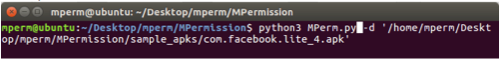
\includegraphics[width=\columnwidth, angle = 0, scale=1.59]{images/screencast/mperm-d.png}
	\caption{M-Perm Reverse Engineering Process}
	\label{fig:mperm-d}
	\end{figure*}
	
	
	
	\item \textbf{Run Analysis Portion:} The analysis portion of M-Perm will only take a few seconds to run, and may be ran using the following command:
	
	\noindent
	\framebox{\parbox{\dimexpr\linewidth-2\fboxsep-2\fboxrule}{\itshape
	\texttt{python3 mperm.py \-a [--analyze] \\ decompiled\_apk\_path}
	}} \\
	
	Figure~\ref{fig:mperm-a} demonstrates the analysis portion of M-Perm.\\
	
	\begin{figure*}[]
	\centering
	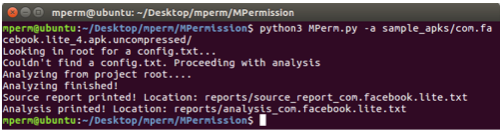
\includegraphics[width=\columnwidth, angle = 0, scale=1.59]{images/screencast/mperm-a.png}
	\caption{Running M-Perm Analysis}
	\label{fig:mperm-a}
	\end{figure*}
	
	
	
	\item \textbf{Analyze Output:} The previous analysis portion of M-Perm produces the output of two .txt files:
	
	\begin{enumerate}
		\item~\texttt{analysis\_<package\_name>}
		\item~\texttt{source\_report\_<package\_name>}
	
	\end{enumerate}
	
	
	
	
	
	These are located in the \emph{reports} directory of M-Perm. A sample output of Facebook Lite \texttt{analysis\_<package\_name>} is shown in Listing 1.
	

%Figure~\ref{lst:MpermOutput1}


	
%	\item \textbf{The first item:} XXXX
%	\item \textbf{The first item:} XXXX


\vspace{30mm}

\lstset{
%numbers=left,
%numberstyle=\small,
%numbersep=8pt,
frame = single,
%language=Pascal,
framexleftmargin=0pt,
framexrightmargin=24pt
}


\begin{lstlisting}[caption=Example M-Perm Output]
---------------- Analysis Report -----
Package: com.facebook.lite

----------- Permissions from Manifest -----
   0 android.permission.READ_CONTACTS
   1 android.permission.CALL_PHONE
   2 com.facebook.receiver.permission.ACCESS
   3 android.permission.WRITE_CALENDAR
   4 android.permission.READ_CALENDAR
   5 android.permission.CHANGE_WIFI_STATE
   6 android.permission.CHANGE_NETWORK_STATE
   7 com.facebook.orca.provider.ACCESS
   8 android.permission.ACCESS_WIFI_STATE
   9 android.permission.INTERNET
  10 com.facebook.lite.permission.C2D_MESSAGE
  .................
\end{lstlisting}
	
	
	%%% ? Talk about how this output may be used?
	
	
\end{enumerate}


\subsection{Installation from Source}

Although using the provided Virtual Machine is recommend, users may install M-Perm from the publicly available source code. M-Perm was written in Python in order to make it as platform independent as possible. Even though we are providing instructions on installing the tool, the user should be cautioned that depending on their platform and configuration, they may be required to install components which are not described in this instruction set. We have tested M-Perm  in Ubuntu 16.04 LTS and OSX 10.10 using Python 3.4.3.

\begin{enumerate}
	\item \textbf{Get Source Code:} The application may be cloned from this Git Repository: https://github.com/dan7800/MPermission.git
	
	
	\item \textbf{Install necessary submodules:} M-Perm uses pre-written decompilation scripts from the kocsenc/android-scraper project. After cloning the project, it can be installed using the following commands:
	
	\noindent
	\framebox{\parbox{\dimexpr\linewidth-2\fboxsep-2\fboxrule}{\itshape
	\texttt{git submodule init}
	}} \\
	 \noindent
	\framebox{\parbox{\dimexpr\linewidth-2\fboxsep-2\fboxrule}{\itshape
	\texttt{git submodule update}
	}} \\
	
	
	\item \textbf{Dependency Set Up:} After cloning and updating the submodule, run:
	
	\noindent
	\framebox{\parbox{\dimexpr\linewidth-2\fboxsep-2\fboxrule}{\itshape
	\texttt{cd android-scraper/tools/apk-decompiler; python3 setupDependencies.py}
	}} \\
	
	Then navigate back to the primary M-Perm directory.\\
	
	\item \textbf{Install Dependencies:} M-Perm's dependencies may be installed using the following command:
	
	\noindent
	\framebox{\parbox{\dimexpr\linewidth-2\fboxsep-2\fboxrule}{\itshape
	\texttt{
	pip install -r requirements.txt}
	}} \\
	
	Note: Depending on your environment and what you have installed, the \texttt{requirements.txt} dependency list may need to be altered.\\
	
	\item \textbf{Run the application:} You should now be able to run M-Perm using the following commands:
		
	\noindent
	\framebox{\parbox{\dimexpr\linewidth-2\fboxsep-2\fboxrule}{\itshape
	\texttt{python3 mperm.py \-d [--decompile] apk\_path}
	}} \\
	
	\noindent
	\framebox{\parbox{\dimexpr\linewidth-2\fboxsep-2\fboxrule}{\itshape
	\texttt{python3 mperm.py \-a [--analyze] \\ decompiled\_apk\_path}
	}} \\


Once completed, follow the instructions to the \emph{Reports} location for the tool's two output files:~\texttt{analysis\_<package\_name>} and~\texttt{source\_report\_<package\_name>} which are located in the \emph{reports} directory of M-Perm.

%	\item \textbf{The first item:} XXXX
%	\item \textbf{The first item:} XXXX
	
	
	
\end{enumerate}



\section{Screen-cast}

\noindent
A link to a screencast of the tool may be found at: \\
%\noindent
%\framebox{\parbox{\dimexpr\linewidth-2\fboxsep-2\fboxrule}{\itshape
\textbf{\url{https://youtu.be/Wz6L2D3dFKs}}
%  }}

%Figure~\ref{fig:architecture}.


\begin{figure}[h]
\centering
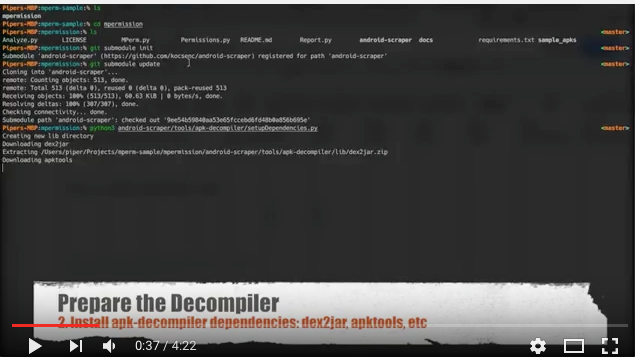
\includegraphics[width=\columnwidth, angle = 0, scale=.99]{images/screencast/youtube.png}
\caption{Youtube Screencast}
\label{fig:youtbuescreencast}
\end{figure}



% A walk through of the actual demonstration, provided as an appendix to the paper (this appendix will not be included in the page count and will not be published).
% A link to a screen-cast or some other accompanying multi-media presentation of the demonstration (if available).
% Information on tool or data availability, maturity and user base, as well as a link to a website for the materials (if one exists) and any tool source code (if open source).



% That's all folks!
\end{document}


% ************************






% Due Date: 6/15/2016
% Guidelines: http://www.cs.ucdavis.edu/fse2016/calls/demos/ 4+1 pages
%


%   Use the term "overprivilege"


% Todo:
%	Create new GH username to make things look cleaner
%   	Create website & domain (LF) - Make things look really pretty. Make sure that case sensitive issues do not exist
%   	Place tool into a virtual machine
% 	APKTool dissassembles. It doesn't decompile
%	Make sure to sell the real value of the tool. Make sure the paper doesn't get lost in other things



%%%%%% Domain Info %%%%%%
% 	https://www.shivarweb.com/2336/namecheap-or-godaddy/


% Submission Info
%	





%%%%%%%%%%%% VM Information  --- Check to make sure that this is correct
% MPerm
% android1234 (all lowercase)

%% Must install GNUNextStep
